\documentclass[11pt,a4paper]{report}
\usepackage[textwidth=37em,vmargin=30mm]{geometry}
\usepackage{calc,xunicode,amsmath,amssymb,paralist,enumitem,tabu,booktabs,datetime2,xeCJK,xeCJKfntef,listings}
\usepackage{tocloft,fancyhdr,tcolorbox,xcolor,graphicx,eso-pic,xltxtra,xelatexemoji}

\newcommand{\envyear}[0]{2024}
\newcommand{\envdatestr}[0]{2024-10-14}
\newcommand{\envfinaldir}[0]{webdb/2024/20241014/final}

\usepackage[hidelinks]{hyperref}
\hypersetup{
    colorlinks=false,
    pdfpagemode=FullScreen,
    pdftitle={Web Digest - \envdatestr}
}

\setlength{\cftbeforechapskip}{10pt}
\renewcommand{\cftchapfont}{\rmfamily\bfseries\large\raggedright}
\setlength{\cftbeforesecskip}{2pt}
\renewcommand{\cftsecfont}{\sffamily\small\raggedright}

\setdefaultleftmargin{2em}{2em}{1em}{1em}{1em}{1em}

\usepackage{xeCJK,xeCJKfntef}
\xeCJKsetup{PunctStyle=plain,RubberPunctSkip=false,CJKglue=\strut\hskip 0pt plus 0.1em minus 0.05em,CJKecglue=\strut\hskip 0.22em plus 0.2em}
\XeTeXlinebreaklocale "zh"
\XeTeXlinebreakskip = 0pt


\setmainfont{Brygada 1918}
\setromanfont{Brygada 1918}
\setsansfont{IBM Plex Sans}
\setmonofont{JetBrains Mono NL}
\setCJKmainfont{Noto Serif CJK SC}
\setCJKromanfont{Noto Serif CJK SC}
\setCJKsansfont{Noto Sans CJK SC}
\setCJKmonofont{Noto Sans CJK SC}

\setlength{\parindent}{0pt}
\setlength{\parskip}{8pt}
\linespread{1.15}

\lstset{
	basicstyle=\ttfamily\footnotesize,
	numbersep=5pt,
	backgroundcolor=\color{black!5},
	showspaces=false,
	showstringspaces=false,
	showtabs=false,
	tabsize=2,
	captionpos=b,
	breaklines=true,
	breakatwhitespace=true,
	breakautoindent=true,
	linewidth=\textwidth
}






\newcommand{\coverpic}[2]{
    % argv: itemurl, authorname
    Cover photo by #2~~(\href{#1}{#1})
}
\newcommand{\makeheader}[0]{
    \begin{titlepage}
        % \newgeometry{hmargin=15mm,tmargin=21mm,bmargin=12mm}
        \begin{center}
            
            \rmfamily\scshape
            \fontspec{BaskervilleF}
            \fontspec{Old Standard}
            \fontsize{59pt}{70pt}\selectfont
            WEB\hfill DIGEST
            
            \vfill
            % \vskip 30pt
            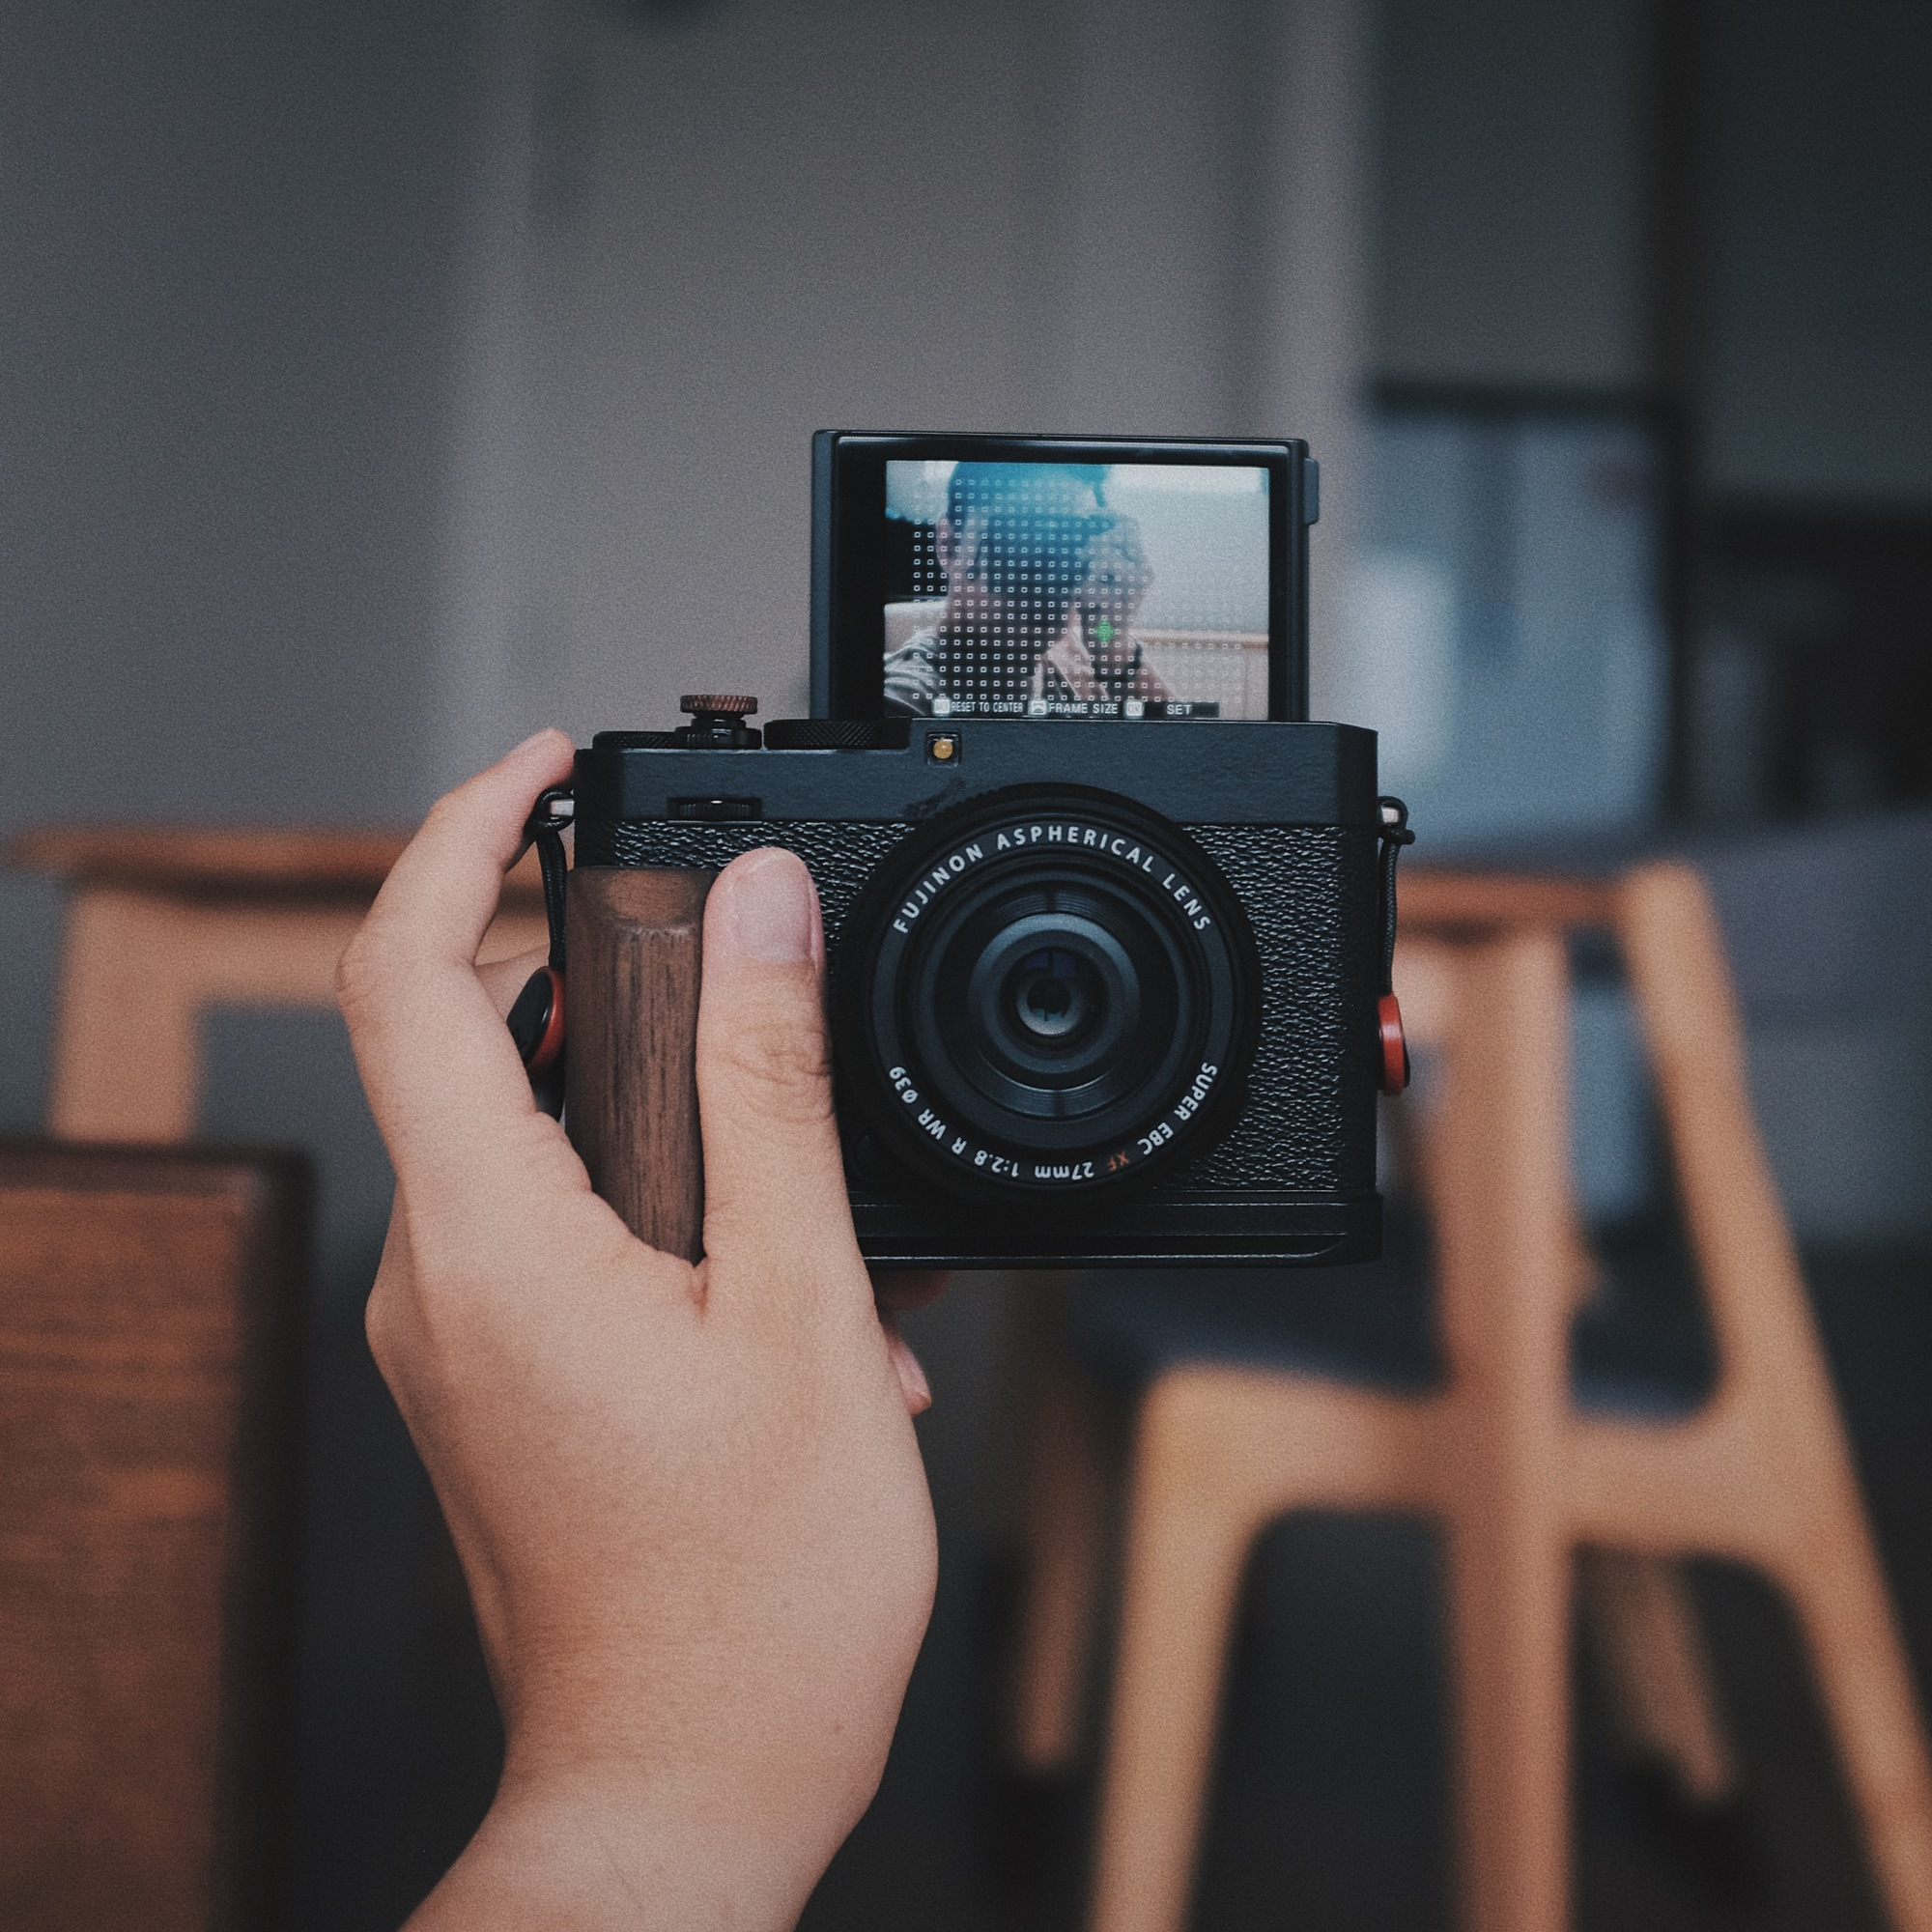
\includegraphics[width=\linewidth]{\envfinaldir/coverpic-prod.jpg}\par
            % \vskip 30pt
            \vfill

            \normalsize\rmfamily\scshape
            \copyright{} The Web Digest Project \hfill\large \envdatestr
        \end{center}
    \end{titlepage}
    % \restoregeometry
}
\newcommand{\simplehref}[1]{%
    \textcolor{blue!80!green}{\href{#1}{#1}}%
}
\renewcommand{\contentsname}{\center\Huge\sffamily\bfseries Contents\par\vskip 20pt}
\newcounter{ipartcounter}
\setcounter{ipartcounter}{0}
\newcommand{\ipart}[1]{
    % \vskip 20pt
    \clearpage
    \stepcounter{ipartcounter}
    \phantomsection
    \addcontentsline{toc}{chapter}{#1}
    % \begin{center}
    %     \Huge
    %     \sffamily\bfseries
    %     #1
    % \end{center}
    % \vskip 20pt plus 7pt
}
\newcounter{ichaptercounter}
\setcounter{ichaptercounter}{0}
\newcommand{\ichapter}[1]{
    % \vskip 20pt
    \clearpage
    \stepcounter{ichaptercounter}
    \phantomsection
    \addcontentsline{toc}{section}{\numberline{\arabic{ichaptercounter}}#1}
    \begin{center}
        \Huge
        \sffamily\bfseries
        #1
    \end{center}
    \vskip 20pt plus 7pt
}
\newcommand{\entrytitlefont}[1]{\subsection*{\raggedright\Large\sffamily\bfseries#1}}
\newcommand{\entryitemGeneric}[2]{
    % argv: title, url
    \parbox{\linewidth}{
        \entrytitlefont{#1}\par\vskip 5pt
        \footnotesize\ttfamily\mdseries
        \simplehref{#2}
    }\vskip 11pt plus 11pt minus 1pt
}
\newcommand{\entryitemGithub}[3]{
    % argv: title, url, desc
    \parbox{\linewidth}{
        \entrytitlefont{#1}\par\vskip 5pt
        \footnotesize\ttfamily\mdseries
        \simplehref{#2}\par\vskip 5pt
        \small\rmfamily\mdseries#3
    }\vskip 11pt plus 11pt minus 1pt
}
\newcommand{\entryitemAp}[3]{
    % argv: title, url, desc
    \parbox{\linewidth}{
        \entrytitlefont{#1}\par\vskip 5pt
        \footnotesize\ttfamily\mdseries
        \simplehref{#2}\par\vskip 5pt
        \small\rmfamily\mdseries#3
    }\vskip 11pt plus 11pt minus 1pt
}
\newcommand{\entryitemHackernews}[3]{
    % argv: title, hnurl, rawurl
    % \parbox{\linewidth}{
    %     \entrytitlefont{#1}\par\vskip 5pt
    %     \footnotesize\ttfamily\mdseries
    %     \simplehref{#3}\par
    %     \textcolor{black!50}{\href{#2}{#2}}
    % }\vskip 11pt plus 11pt minus 1pt
    \begin{minipage}{\linewidth}
            \entrytitlefont{#1}\par\vskip 5pt
            \footnotesize\ttfamily\mdseries
            \simplehref{#3}\par
            \textcolor{black!50}{\href{#2}{#2}}
    \end{minipage}\par\vskip 11pt plus 11pt minus 1pt
}







\begin{document}

\makeheader

\tableofcontents\clearpage




\ipart{Developers}
\ichapter{Hacker News}
\entryitemTwoLinks{CRLF is obsolete and should be abolished}{https://news.ycombinator.com/item?id=41830717}{https://fossil-scm.org/home/ext/crlf-harmful.md}

\entryitemTwoLinks{Making the Tibetan language a first-class citizen in the digital world}{https://news.ycombinator.com/item?id=41829926}{https://www.bdrc.io/blog/2024/10/10/tech-innovations-to-make-the-tibetan-language-a-first-class-citizen-in-the-digital-world/}

\entryitemTwoLinks{Restic: Backups done right}{https://news.ycombinator.com/item?id=41829913}{https://restic.net/}

\entryitemTwoLinks{ACF Plugin no longer available on WordPress.org}{https://news.ycombinator.com/item?id=41828958}{https://www.advancedcustomfields.com/blog/acf-plugin-no-longer-available-on-wordpress-org/}

\entryitemTwoLinks{Ward Christensen (of BBS and XMODEM fame) has died}{https://news.ycombinator.com/item?id=41828923}{https://en.wikipedia.org/wiki/Ward\_Christensen}

\entryitemTwoLinks{America's new millionaire class: Plumbers and HVAC entrepreneurs}{https://news.ycombinator.com/item?id=41828896}{https://www.wsj.com/business/entrepreneurship/plumbers-hvac-skilled-trades-millionaires-2b62bf6c}

\entryitemTwoLinks{The quiet art of attention}{https://news.ycombinator.com/item?id=41828601}{https://billwear.github.io/art-of-attention.html}

\entryitemTwoLinks{Starship Flight 5: Launch and booster catch [video]}{https://news.ycombinator.com/item?id=41827362}{https://twitter.com/SpaceX/status/1845152255944819015}

\entryitemTwoLinks{Large language models reduce public knowledge sharing on online Q\&A platforms}{https://news.ycombinator.com/item?id=41827043}{https://academic.oup.com/pnasnexus/article/3/9/pgae400/7754871}

\entryitemTwoLinks{Eating less can lead to a longer life: study in mice shows why}{https://news.ycombinator.com/item?id=41826449}{https://www.nature.com/articles/d41586-024-03277-6}

\entryitemTwoLinks{Diffusion for World Modeling}{https://news.ycombinator.com/item?id=41826402}{https://diamond-wm.github.io/}

\entryitemTwoLinks{WordPress.org's latest move involves taking control of a WP Engine plugin}{https://news.ycombinator.com/item?id=41826082}{https://www.theverge.com/2024/10/12/24268637/wordpress-org-matt-mullenweg-acf-fork-secure-custom-fields-wp-engine}

\entryitemTwoLinks{ACF has been hijacked}{https://news.ycombinator.com/item?id=41824852}{https://anderegg.ca/2024/10/13/acf-has-been-hijacked}

\entryitemTwoLinks{FLUX is fast and it's open source}{https://news.ycombinator.com/item?id=41824390}{https://replicate.com/blog/flux-is-fast-and-open-source}

\entryitemTwoLinks{Omni SenseVoice: High-Speed Speech Recognition with Words Timestamps}{https://news.ycombinator.com/item?id=41824171}{https://github.com/lifeiteng/OmniSenseVoice}

\entryitemTwoLinks{The 1/8th Sleep}{https://news.ycombinator.com/item?id=41824138}{https://near.blog/the-1-8th-sleep/}

\entryitemTwoLinks{First Greenhouse Gas Plumes Detected with NASA-Designed Instrument}{https://news.ycombinator.com/item?id=41822321}{https://www.jpl.nasa.gov/news/first-greenhouse-gas-plumes-detected-with-nasa-designed-instrument/}

\entryitemTwoLinks{Show HN: AOO – C++ library for real-time audio streaming and messaging}{https://news.ycombinator.com/item?id=41822303}{https://aoo.iem.sh/}

\entryitemTwoLinks{PayPal (USA) will automatically share data about you to participating stores}{https://news.ycombinator.com/item?id=41822178}{https://www.paypal.com/us/legalhub/upcoming-policies-full}

\entryitemTwoLinks{Ask HN: If you were rewriting Emacs from scratch, what would you do differently?}{https://news.ycombinator.com/item?id=41821545}{https://news.ycombinator.com/item?id=41821545}\ichapter{Phoronix}
\entryitemGeneric{\hskip 0pt{}Linux 6.12-rc3 Released With Some Late NTFS Driver Enhancements}{https://www.phoronix.com/news/Linux-6.12-rc3-Released}

\entryitemGeneric{\hskip 0pt{}Linux 6.13 To Drop Some Old \& No Longer Maintained Staging Drivers}{https://www.phoronix.com/news/Linux-6.13-Dropping-Old-Drivers}

\entryitemGeneric{\hskip 0pt{}Improvements To The Ad Experience}{https://www.phoronix.com/news/Improving-Ad-Experience-2024}

\entryitemGeneric{\hskip 0pt{}Mesa 24.3 Allows Rusticl On Asahi Gallium3D By Default}{https://www.phoronix.com/news/Rusticl-Asahi-Default-Mesa-24.3}

\entryitemGeneric{\hskip 0pt{}Mesa NVK Vulkan Driver Adds VK\_KHR\_fragment\_shading\_rate Support}{https://www.phoronix.com/news/NVK-Fragment-Shading-Rate}

\entryitemGeneric{\hskip 0pt{}Microsoft's Azure Linux 2.0 Updated With Dozens Of Security Fixes}{https://www.phoronix.com/news/Azure-Linux-2.0.20241006}

\entryitemGeneric{\hskip 0pt{}Wayland Protocols 1.38 Brings System Bell, FIFO \& Commit Timing Protocols}{https://www.phoronix.com/news/Wayland-Protocols-1.38}

\entryitemGeneric{\hskip 0pt{}AMD XDNA Linux Driver Updated As It Nears The Upstream Kernel}{https://www.phoronix.com/news/AMD-XDNA-Linux-Driver-v4}

\entryitemGeneric{\hskip 0pt{}BeOS-Inspired Haiku Enabling More Intel Hardware \& Driving Kernel Optimizations}{https://www.phoronix.com/news/Haiku-OS-September-2024}


\ipart{Developers~~~~(zh-Hans)}
\ichapter{Solidot}
\entryitemGeneric{\hskip 0pt{}志愿者想要保护维基百科免遭 AI 生成内容的入侵}{https://www.solidot.org/story?sid=79476}

\entryitemGeneric{\hskip 0pt{}上交所通过重启系统解决堵单问题}{https://www.solidot.org/story?sid=79475}

\entryitemGeneric{\hskip 0pt{}美国肥胖率开始下降}{https://www.solidot.org/story?sid=79474}

\entryitemGeneric{\hskip 0pt{}男子通过苹果 AI 的短信总结获悉分手的消息}{https://www.solidot.org/story?sid=79473}

\entryitemGeneric{\hskip 0pt{}苹果研究员发现大模型不能形式推理}{https://www.solidot.org/story?sid=79472}

\entryitemGeneric{\hskip 0pt{}Google 准备让用户在 Android 上运行 Linux 应用}{https://www.solidot.org/story?sid=79471}

\entryitemGeneric{\hskip 0pt{}广东教育厅短信平台被黑客入侵群发成人电影网站链接}{https://www.solidot.org/story?sid=79470}

\entryitemGeneric{\hskip 0pt{}科沃斯扫地机器人被黑客入侵发表种族歧视或仇恨言论}{https://www.solidot.org/story?sid=79469}

\entryitemGeneric{\hskip 0pt{}Steam 告诉玩家购买的是许可证并不真的拥有游戏}{https://www.solidot.org/story?sid=79468}

\entryitemGeneric{\hskip 0pt{}Mozilla 刚修复的 0day 被用于攻击 Tor 浏览器用户}{https://www.solidot.org/story?sid=79467}

\entryitemGeneric{\hskip 0pt{}Fedora Asahi Remix 支持运行部分 3A 游戏}{https://www.solidot.org/story?sid=79466}

\entryitemGeneric{\hskip 0pt{}网信办展开规范网络语言文字专项行动}{https://www.solidot.org/story?sid=79465}

\entryitemGeneric{\hskip 0pt{}X-37B 将执行一系列机动}{https://www.solidot.org/story?sid=79464}

\entryitemGeneric{\hskip 0pt{}诺贝尔和平奖授予日本核爆受害者团体}{https://www.solidot.org/story?sid=79463}

\entryitemGeneric{\hskip 0pt{}调查发现父母更信任 ChatGPT 生成的健康指导}{https://www.solidot.org/story?sid=79462}

\entryitemGeneric{\hskip 0pt{}Google 量子计算机能打败今天最强的超算}{https://www.solidot.org/story?sid=79461}

\entryitemGeneric{\hskip 0pt{}哆啦A梦声优大山羡代去世}{https://www.solidot.org/story?sid=79460}

\entryitemGeneric{\hskip 0pt{}英特尔宣布了酷睿 Ultra 200 系列桌面处理器}{https://www.solidot.org/story?sid=79459}

\entryitemGeneric{\hskip 0pt{}研究称盗版会导致游戏收益损失 19\%}{https://www.solidot.org/story?sid=79458}

\entryitemGeneric{\hskip 0pt{}黑客入侵美国 ISP 访问后门系统证明苹果关于加密后门的观点是正确的}{https://www.solidot.org/story?sid=79457}\ichapter{V2EX}
\entryitemGeneric{\hskip 0pt{}[RSS] 关注网络安全资讯的 follow list}{https://www.v2ex.com/t/1079911}

\entryitemGeneric{\hskip 0pt{}[分享发现] 见证历史! SpaceX 星舰第 5 次试飞 筷子塔成功捕获!}{https://www.v2ex.com/t/1079910}

\entryitemGeneric{\hskip 0pt{}[NAS] 群晖 DS423+ NVME SSD 速度极慢!}{https://www.v2ex.com/t/1079909}

\entryitemGeneric{\hskip 0pt{}[iOS] 无忧行 url schema 参数}{https://www.v2ex.com/t/1079907}

\entryitemGeneric{\hskip 0pt{}[Reddit] 为什么 reddit 上中文板块这么少}{https://www.v2ex.com/t/1079906}

\entryitemGeneric{\hskip 0pt{}[宽带症候群] 找 IDC 或运营商宽带资源}{https://www.v2ex.com/t/1079905}

\entryitemGeneric{\hskip 0pt{}[问与答] 微信永封后仍然从微信支付中自动扣费,是否违规,是否可追回}{https://www.v2ex.com/t/1079904}

\entryitemGeneric{\hskip 0pt{}[分享发现] Netflix(网飞)2024 部分电影和剧集分享,持续更新}{https://www.v2ex.com/t/1079903}

\entryitemGeneric{\hskip 0pt{}[游戏] 杀戳尖塔怎么感觉爽不起来?}{https://www.v2ex.com/t/1079901}

\entryitemGeneric{\hskip 0pt{}[分享创造] CloudFlare 临时邮箱 也可注册账号绑定邮箱}{https://www.v2ex.com/t/1079900}

\entryitemGeneric{\hskip 0pt{}[宽带症候群] 爬墙还跟光猫有关吗}{https://www.v2ex.com/t/1079899}

\entryitemGeneric{\hskip 0pt{}[问与答] 你有什么高效的用手机背单词的方法吗?}{https://www.v2ex.com/t/1079898}

\entryitemGeneric{\hskip 0pt{}[Apple] iPhone16PM 游戏和散热性能实际体验小感受}{https://www.v2ex.com/t/1079897}

\entryitemGeneric{\hskip 0pt{}[iCloud] Apple 土区 iCloud 2T 5 人车 已开 2 年}{https://www.v2ex.com/t/1079896}

\entryitemGeneric{\hskip 0pt{}[问与答] 35 岁 初中学历怎么提升学历?}{https://www.v2ex.com/t/1079895}

\entryitemGeneric{\hskip 0pt{}[macOS] macOS 版的 WPS 更新,支持最新的窗口管理功能, Moom 卸载咯!}{https://www.v2ex.com/t/1079894}

\entryitemGeneric{\hskip 0pt{}[程序员] 小 心 任 何 二 次 接 手 的 代 码}{https://www.v2ex.com/t/1079893}

\entryitemGeneric{\hskip 0pt{}[Go 编程语言] 在本地快速构建微服务集群(秒杀抢购和订单功能)来验证测试,个人感觉使用 dtm 来解决分布式事务还是挺优雅的,而且使用也比较简单。}{https://www.v2ex.com/t/1079891}

\entryitemGeneric{\hskip 0pt{}[宽带症候群] 关于接了三网之后的事情}{https://www.v2ex.com/t/1079890}

\entryitemGeneric{\hskip 0pt{}[问与答] 为什么总是记住坏事忘记好事,是什么毛病?}{https://www.v2ex.com/t/1079889}

\entryitemGeneric{\hskip 0pt{}[分享创造] 我创建了一个 AI 驱动的社交互动助手网站 - RizzLinesAI}{https://www.v2ex.com/t/1079888}

\entryitemGeneric{\hskip 0pt{}[iPhone] 关于 16pro 屏幕混用}{https://www.v2ex.com/t/1079885}

\entryitemGeneric{\hskip 0pt{}[宽带症候群] 换成 IPoE 的朋友来说一下体验怎么样?桥接?公网 IP?软路由?}{https://www.v2ex.com/t/1079882}

\entryitemGeneric{\hskip 0pt{}[职场话题] 各位现在过的如何?}{https://www.v2ex.com/t/1079881}

\entryitemGeneric{\hskip 0pt{}[问与答] 人生的意义是什么。}{https://www.v2ex.com/t/1079880}

\entryitemGeneric{\hskip 0pt{}[问与答] windows 哪个录屏软件好用 ?}{https://www.v2ex.com/t/1079879}

\entryitemGeneric{\hskip 0pt{}[问与答] 怎么查看 ssh 回显延迟}{https://www.v2ex.com/t/1079877}

\entryitemGeneric{\hskip 0pt{}[宽带症候群] 宽带仅有 ipv6,无法获取 ipv4}{https://www.v2ex.com/t/1079876}

\entryitemGeneric{\hskip 0pt{}[问与答] 为啥有些开发者开发出产品以后会宣传自己开发过程中有多么艰辛,晚上睡不着,头发掉了多少根}{https://www.v2ex.com/t/1079875}

\entryitemGeneric{\hskip 0pt{}[职场话题] 好像经历了什么套路裁员}{https://www.v2ex.com/t/1079874}

\entryitemGeneric{\hskip 0pt{}[问与答] 有没有将视频倒放的播放器}{https://www.v2ex.com/t/1079873}

\entryitemGeneric{\hskip 0pt{}[问与答] 中国电信计划在 2024 年内收回所有老用户的公网 IPv4?}{https://www.v2ex.com/t/1079872}

\entryitemGeneric{\hskip 0pt{}[程序员] 鸿蒙的 helloworld 第一天就被劝退}{https://www.v2ex.com/t/1079871}

\entryitemGeneric{\hskip 0pt{}[问与答] 求推荐老人防走失定位设备}{https://www.v2ex.com/t/1079870}

\entryitemGeneric{\hskip 0pt{}[Apple] mba m3 触控 id 键按下锁屏不灵敏,有 v 友遇到过吗}{https://www.v2ex.com/t/1079869}

\entryitemGeneric{\hskip 0pt{}[SpaceX] 星舰第五次 发射,被 🥢 拿捏夹住了!}{https://www.v2ex.com/t/1079868}

\entryitemGeneric{\hskip 0pt{}[分享创造] 开发了一个识别浏览器环境的网站: BrowserIs}{https://www.v2ex.com/t/1079864}

\entryitemGeneric{\hskip 0pt{}[iPhone] 寻找视频转实况照片的工具}{https://www.v2ex.com/t/1079863}

\entryitemGeneric{\hskip 0pt{}[iPhone] 60Hz 有一个 Promotion 没有的优势}{https://www.v2ex.com/t/1079862}

\entryitemGeneric{\hskip 0pt{}[生活] 因为工作难找而创业,必然是一个更难且费钱的选择,我选择离婚、背债、流浪汉}{https://www.v2ex.com/t/1079861}

\entryitemGeneric{\hskip 0pt{}[问与答] V 友会不会经常忘记自己去过的地方或吃过的东西?}{https://www.v2ex.com/t/1079860}

\entryitemGeneric{\hskip 0pt{}[问与答] v2 移动端客户端选择}{https://www.v2ex.com/t/1079859}

\entryitemGeneric{\hskip 0pt{}[问与答] EDGE 的侧边栏搜索,无法修改默认 cn.bing.com,哪里可以设置吗?}{https://www.v2ex.com/t/1079858}

\entryitemGeneric{\hskip 0pt{}[Apple] 靠谱的 iPhone 屏幕维修和换电池}{https://www.v2ex.com/t/1079856}

\entryitemGeneric{\hskip 0pt{}[问与答] phper 提桶跑路后转行家具维修行业后的一些感触}{https://www.v2ex.com/t/1079855}

\entryitemGeneric{\hskip 0pt{}[Linux] 有使用 NextCloud 的朋友吗? 问一下 [服务器端加密] 功能,是开了就自动加密,解密就是用户密码对吧?}{https://www.v2ex.com/t/1079852}

\entryitemGeneric{\hskip 0pt{}[ WATCH] 在 watch 上点开和联系人的信息都是短信,同时在 iPhone 上是 iMessage,有大佬知道怎么解决吗?}{https://www.v2ex.com/t/1079851}

\entryitemGeneric{\hskip 0pt{}[职场话题] 请教大家记录 Teams 或 Zoom 会议语音转文本都用什么软件}{https://www.v2ex.com/t/1079850}

\entryitemGeneric{\hskip 0pt{}[程序员] 一个很老的话题,但还是想问问大家,后端搞前端怎么选}{https://www.v2ex.com/t/1079848}

\entryitemGeneric{\hskip 0pt{}[游戏] 一个用 Vanilla HTML/JS 当 UI 的游戏 Universal Paperclips}{https://www.v2ex.com/t/1079847}


\ipart{Generic News}
\ichapter{AP News}
\entryitemWithDescription{\hskip 0pt{}Patriots captain Jabrill Peppers arrested on assault, strangulation, drug charges}{https://apnews.com/article/344c01120bd470b457c3c2bdef065d81}{}\ichapter{Reuters}
\entryitemWithDescription{\hskip 0pt{}Man arrested near Trump rally in California on gun charges}{https://www.reuters.com/world/us/man-arrested-near-trump-rally-california-gun-charges-2024-10-13/}{The man, arrested on Saturday, was charged with possession of a loaded firearm and possession of a high-capacity...}

\entryitemWithDescription{\hskip 0pt{}World Bank says 26 poorest countries in worst financial shape since 2006}{https://www.reuters.com/world/world-bank-says-26-poorest-countries-worst-financial-shape-since-2006-2024-10-13/}{The world\textquotesingle s 26 poorest countries, home to 40\% of the most poverty-stricken people, are more in debt than at any time since 2006 and increasingly vulnerable to natural disasters and other shocks, a new World Bank report...}

\entryitemWithDescription{\hskip 0pt{}UN chief says any attacks on Lebanon peacekeepers could be a war crime}{https://www.reuters.com/world/un-chief-says-any-attacks-lebanon-peacekeepers-could-be-war-crime-2024-10-13/}{United Nations Secretary-General Antonio Guterres warned on Sunday that any attacks against peacekeepers "may constitute a war crime," his spokesperson said after Israeli tanks burst through the gates of a peacekeeping base in southern...}

\entryitemWithDescription{\hskip 0pt{}Albania's prime minister sees CEFTA progress for Western Balkans}{https://www.reuters.com/world/europe/albanias-prime-minister-sees-cefta-progress-western-balkans-2024-10-13/}{Albanian Prime Minister Edi Rama said on Sunday that an enhanced Central European Free Trade Agreement (CEFTA) for the Western Balkan region was within reach as his country seeks to make itself fit for membership of the European Union by...}

\entryitemWithDescription{\hskip 0pt{}Zelenskiy says North Koreans fighting with Russians in Ukraine}{https://www.reuters.com/world/europe/zelenskiy-says-north-koreans-fighting-with-russians-ukraine-2024-10-13/}{Ukrainian President Volodymyr Zelenskiy said on Sunday that defence relationships with his country\textquotesingle s partners would have to change in light of North Korean transfers of people as well as weapons to Russian forces in...}

\entryitemWithDescription{\hskip 0pt{}Italy's Intesa Sanpaolo apologises for security breach involving PM Meloni}{https://www.reuters.com/world/europe/italys-intesa-sanpaolo-apologises-security-breach-involving-pm-meloni-2024-10-13/}{Italy\textquotesingle s biggest bank Intesa Sanpaolo apologised on Sunday for an embarrassing security breach that reportedly targeted Prime Minister Giorgia Meloni and other high-profile...}

\entryitemWithDescription{\hskip 0pt{}Lebanon's Hezbollah said it launched drone attack on north Israeli town}{https://www.reuters.com/world/middle-east/lebanons-hezbollah-said-it-launched-drone-attack-north-israeli-town-2024-10-13/}{Lebanon\textquotesingle s militant group Hezbollah said in a statement that it attacked a Golani Brigade camp in the northern Israeli town of Binyamina with a "swarm of drones" on...}

\entryitemWithDescription{\hskip 0pt{}NASA spacecraft to study whether Jupiter's moon Europa can harbor life}{https://www.reuters.com/technology/space/nasa-spacecraft-study-whether-jupiters-moon-europa-can-harbor-life-2024-10-13/}{Observations hint at a vast underground ocean below Europa\textquotesingle s icy...}

\entryitemWithDescription{\hskip 0pt{}Iceland PM dissolves parliament and calls elections, RUV reports}{https://www.reuters.com/world/europe/iceland-pm-announces-end-governing-coalition-ruv-reports-2024-10-13/}{Elections must take place at the latest 45 days after the dissolution of parliament is announced, the broadcaster...}

\entryitemWithDescription{\hskip 0pt{}US to send anti-missile system to Israel, says Pentagon}{https://www.reuters.com/world/us-send-anti-missile-system-israel-says-pentagon-2024-10-13/}{U.S. troops will operate the...}

\entryitemWithDescription{\hskip 0pt{}Under bombardment, Lebanon's expectant mothers fear for their unborn babies}{https://www.reuters.com/world/middle-east/under-bombardment-lebanons-expectant-mothers-fear-their-unborn-babies-2024-10-13/}{Tahani Yassine was in her third trimester of pregnancy when she chose to return to her hometown of Beirut to deliver her...}

\entryitemWithDescription{\hskip 0pt{}Thousands march in Spain to demand affordable housing}{https://www.reuters.com/world/europe/thousands-march-spain-demand-affordable-housing-2024-10-13/}{Thousands protested on Sunday in Madrid to demand more affordable housing amid rising anger from Spaniards who feel they are being priced out of the...}

\entryitemWithDescription{\hskip 0pt{}SpaceX catches giant Starship booster in fifth flight test}{https://www.reuters.com/technology/space/spacex-launches-fifth-starship-test-eyes-novel-booster-catch-2024-10-13/}{The company achieved another novel engineering feat in its push to build a reusable moon and Mars...}\ichapter{联合早报}
\entryitemWithDescription{沈泽玮:台湾冲突阻遏法案只叫不咬?}{https://www.zaobao.com/news/china/story20240918-4758889}{美国众议院9月9日开启了长达一星期的``中国周'',共通过25项主要涉华法案。(法新社) 美国众议院在当地时间9月9日开启了长达一星期的``中国周'',在美国总统和国会选举举行之前,密集表决数十项与中国有关的法案,共通过25项主要涉华法案……}

\entryitemWithDescription{欧盟电动车关税投票倒计时 中国在分歧中寻支持}{https://www.zaobao.com/news/china/story20240917-4758953}{欧盟27个成员国将于9月25日就是否继续对进口自中国的电动汽车额外征税进行最后表决。图为上海港等待装运出口的电动汽车。(彭博社) 欧盟对中国电动汽车加征关税的投票进入倒计时,正在欧洲访问的中国商务部部长王文涛与欧盟多国政府高层就此进行协商,试图在立场分歧的成员国中争取到更多支持。 受访学者研判,欧盟对中国电动汽车加征关税不可避免,但具体的加税方式和幅度仍有一定弹性,这是王文涛此行与各国谈判的重点……}

\entryitemWithDescription{港府今年将举办逾400项国庆活动}{https://www.zaobao.com/news/china/story20240917-4759341}{再过十多天就是中国国庆75周年,香港天星小轮展示``国庆75周年''\,``三天免费搭小轮''等标语迎国庆。(中新社) 再过十多天就是中国国庆75周年,香港特区政府今年将举办逾400项庆祝活动,希望通过一连串活动庆祝国庆,并且弘扬爱国主义教育及刺激消费。 港府星期二(9月17日)召开记者会,介绍各项庆祝国庆活动和特别优惠,涉及出行及吃喝玩乐等领域……}

\entryitemWithDescription{美空军部长:中国大陆军演精密化 为入侵封锁台湾做准备}{https://www.zaobao.com/news/china/story20240917-4759407}{美国空军部长肯德尔星期一(9月16日)在空军暨太空军协会的一场大会上致辞,提到中国对印太地区日益增长的威胁。(取自美国国防部网站) (华盛顿综合讯)美国空军部长肯德尔指,中国大陆军演的规模越来越大,也更加精密化,这是在专门为入侵、封锁台湾做准备。他也称,中国对印太地区的威胁现在已存在……}

\entryitemWithDescription{批准潜在对台备件军售案后 美派巡逻机过航台海}{https://www.zaobao.com/news/china/story20240917-4758770}{台军士兵8月26日在屏东县枋山训练场进行实弹演习时,从M1167 TOW运载车上发射一枚美制TOW-2A线导反坦克导弹。(路透社) (华盛顿/台北/北京综合讯)在批准潜在对台备件军售案之后,美国派遣反潜巡逻机过航台湾海峡,中国人民解放军东部战区则组织战机跟监美机,并誓言``坚决捍卫国家主权''……}

\entryitemWithDescription{李家超:若香港驻美经贸办被关 受害的是美企}{https://www.zaobao.com/news/china/story20240917-4758797}{香港特首李家超星期一(9月17日)警告,如果美国通过法案,导致香港驻美经贸办关闭,受害的是美国企业。图为李家超9月11日在``一带一路''高峰论坛上致辞。(彭博社) (香港综合讯)香港特首李家超警告,如果美国通过法案,导致香港驻美经贸办关闭,受害的是美国企业。 美国众议院上周通过《香港经济贸易办事处认证法案》,如果参议院也表决通过并交由总统签署成法,香港三个驻美国的经贸办可能将被强制关闭……}

\entryitemWithDescription{美国指中国航空工业集团员工企图实施黑客攻击}{https://www.zaobao.com/news/china/story20240917-4757988}{(华盛顿综合讯)中国航空航天巨头中国航空工业集团一名员工被指试图对美国宇航局、美国军方和其他目标展开黑客攻击。 据彭博社报道,美国检察官布坎南星期一(9月16日)在起诉书中,指控中国航空工业集团39岁的工程师吴宋(音译,Song Wu)企图从美国宇航局、空军、陆军和海军,以及联邦航空管理局取得电脑软件和源代码……}

\entryitemWithDescription{【东谈西论】恒大账务造假 普华永道是共犯还是被拖累?}{https://www.zaobao.com/news/china/story20240917-4756452}{因涉及恒大地产审计项目的违法行为,普华永道中国9月13日被中国财政部和证监会处以4.41亿人民币罚款并被令停业六个月, 广州分所被撤销……}

\entryitemWithDescription{戴庆成:香港输入人才计划大检阅}{https://www.zaobao.com/news/china/story20240917-4744978}{香港于2022年底推出高端人才通行证计划。(法新社) 2019年香港反修例风波过后,数以十万计港人移居海外,令香港出现人才荒。港府为了解决这个问题,在过去几年积极引入``新血'',当中以高才通计划最受瞩目,社会上也不时热议其成效。 高才通全称为高端人才通行证计划,于2022年底推出,申请人年收入须达到250万港元(约42万新元)以上,或本科毕业于全球百强大学并满足一定工作年限等……}

\entryitemWithDescription{中美希望稳定双边关系 中小国家可​​​搭建桥梁}{https://www.zaobao.com/news/china/story20240917-4745091}{中美元首去年11月在旧金山会晤后,双方都希望稳定两国关系,我国巡回大使陈庆珠认为,如果中美两国都认为走向战争不符合它们的利益,那么中小国家就可以做点什么,为双方搭建桥梁。 陈庆珠星期一(9月16日)在李光耀公共政策学院的一场研讨会上说,中国与西方的关系面对诸多困难,有中国智库表示,希望新加坡能协助在中美之间建立更多对话,``因为新加坡受美国信任,也在中国有渠道''……}

\entryitemWithDescription{陈庆珠:世界经历了三次``中国冲击'' 中美的主导力之争将继续}{https://www.zaobao.com/news/china/story20240917-4744996}{李光耀公共政策学院``思想之节庆''的一场研讨会,讨论``历史终结时的中国冲击''。左起是我国巡回大使陈庆珠、通商中国主席李奕贤、李光耀公共政策学院国际关系助理教授何莉菁、李光耀公共政策学院院长柯成兴……}

\entryitemWithDescription{上海遭遇75年来最强台风 扰乱民众中秋假期出行}{https://www.zaobao.com/news/china/story20240916-4745224}{台风贝碧嘉星期一(9月16日)登陆上海,维护人员星期一下午在衡山路上处理倒伏的树木。 (新华社) 台风造成上海上万株数目倒伏或折断。图为一棵倒下的大树砸坏一旁的建筑。(法新社) 台风贝碧嘉登陆上海后,黄浦江苏州河口潮位上涨,乌云密布。(中新社) 中国上海市星期一(9月16日)遭遇75年来最强台风``贝碧嘉''登陆,也是上海有记录以来首次有强台风侵袭……}

\entryitemWithDescription{陆男频长驱偷渡台湾在测试边防实力?}{https://www.zaobao.com/news/china/story20240916-4745161}{中国大陆一名王姓男子在中秋节前夕,乘橡皮艇从浙江宁波抵达台湾新北市林口,主动打电话投案,海巡署人员前去接他上岸。(自由時報) 中国大陆一名王姓男子划橡皮艇于上星期六清晨偷渡到台湾,隔天被新北市地方法院裁定羁押禁见。这是6月以来第二起大陆人士偷渡至台湾,此间专家质疑是否为海防破口,并怀疑对岸是否在测试台湾的边防实力……}

\entryitemWithDescription{中美时隔八月举行国防部工作会晤}{https://www.zaobao.com/news/china/story20240916-4745025}{(北京/华盛顿综合讯)中美双方上周末举行国防部工作会晤;美国官员称,美国积极进行美中两军外交活动,不代表美国对有关中国议题的处理方式发生任何改变。 据中国国防部星期天(15日)晚上通报,北京香山论坛结束后,第18次中美国防部工作会晤上星期六至星期天(9月14日至15日)在北京举行……}

\entryitemWithDescription{中国高校今年拟增足球运动本科专业}{https://www.zaobao.com/news/china/story20240916-4744925}{(北京综合讯)为了培养足球专业人才,中国大专学府今年度拟新增足球运动本科专业,以具体落实中国足球改革。 综合人民网和《南方都市报》报道,中国教育部上星期五(9月13日)发布《2024年度普通高等学校本科专业申报材料公示》。根据公示统计,今年度拟新增专业535个,涉及353所高校,其中39所高校新增足球运动专业……}

\entryitemWithDescription{香港23条首案 港男因穿``光时''上衣被定罪}{https://www.zaobao.com/news/china/story20240916-4743439}{(香港综合讯)香港一名无业男子,今年6月因穿印有2019年反修例抗争口号的上衣而被捕。他星期一承认违反煽动意图罪,成为在《维护国家安全条例》(即《香港基本法》第23条)下被定罪的第一人。 综合港媒《星岛日报》和路透社报道,27岁无业男子诸启邦今年6月12日在石门港铁站附近,未能出示身份证供查阅被警方拘捕……}

\entryitemWithDescription{美国务院:中国释放被关押近20年美籍牧师}{https://www.zaobao.com/news/china/story20240916-4744614}{(华盛顿综合电)中国释放被关押近20年的美国籍牧师,显示北京在中美关系的关键时刻展现善意。 综合彭博社、法新社和路透社报道,美国国务院发言人星期天(9月15日)说:``我们欢迎林大卫(音译,David Lin)从中华人民共和国的监狱获释。他已回返美国,这是他近20年来首次与家人见面。'' 林大卫的女儿艾丽斯告诉美国政治新闻网Politico,她的父亲将抵达得克萨斯州的圣安东尼奥……}

\entryitemWithDescription{中国驻泰使馆:近期并未向湄公河下游泄洪}{https://www.zaobao.com/news/china/story20240916-4743917}{(北京讯)泰国西北部的湄公河因洪水泛滥而决堤,中国否认这是中方泄洪所致,并称近来已持续减少云南景洪水电站的出库流量,以助下游地区抗洪。 中国驻泰国大使馆星期日(9月15日)深夜在官方微信公众号发文说,当天又有媒体报道称中国正在向湄公河泄洪,经向中国主管部门核实,使馆再次澄清,为帮助下游地区应对洪灾,中方近来持续稳定和减少景洪水电站出库流量,不可能对下游地区抗洪救灾形成压力……}

\entryitemWithDescription{加入美国储存可靠度评估计划 台湾军方编列预算采购三类型导弹}{https://www.zaobao.com/news/china/story20240916-4743826}{(台北讯)据台媒报道,台湾军方持续向美国采购可简易操作的导弹,预计在2024年、2031年以前获得400枚``标枪''反装甲导弹、2485枚``刺针''人携式防空导弹……}

\entryitemWithDescription{韩咏红:中美分头追逐全球南方}{https://www.zaobao.com/news/china/story20240916-4730719}{9月5日,中国外长王毅(中)同中非合作论坛非方现任共同主席国塞内加尔外长法勒(左)、下任共同主席国刚果外长加科索(右),在北京共同会见中外记者并答问。(路透社) 进入气候宜人的9月,中国接连举行了两场受瞩目的国际会议,一是聚集非洲53国国家元首与政要的中非合作论坛,接着是周末刚闭幕的北京香山论坛。 两场活动的参与者不同,规模也有很大差距……}

\entryitemWithDescription{菲律宾船只撤离中菲争议海域后 将再派船接替}{https://www.zaobao.com/news/china/story20240915-4730494}{这张在9月15日拍摄,并由菲律宾海岸警卫队提供的照片显示,菲律宾海岸警卫队船马格巴努亚号抵达了菲国巴拉望岛的一个港口。菲律宾早前以发现填海活动为由,今年4月派出马格巴努亚号前往萨比纳礁。(法新社/菲律宾海岸警卫队) 菲律宾国家海事委员会星期天(9月15日)发声明称,该国海岸警卫队一艘巡逻舰已离开萨比纳礁争议海域……}

\entryitemWithDescription{台风贝碧嘉直击中国华东 多趟本地与沪杭间航班取消}{https://www.zaobao.com/news/china/story20240915-4730611}{9月15日在上海外滩滨江步道上,一名外籍游客的雨伞被大风吹起。台风贝碧嘉的中心当天下午5时位于上海市东偏南方大约435公里的东海海面上,中心附近最大风力有13级。(中新社) (上海/新加坡综合讯)台风贝碧嘉预计将为中国华东沿海地区带来狂风暴雨,多趟往返新加坡与上海和杭州的航班取消……}






\clearpage
\leavevmode\vfill
\footnotesize

Copyright \copyright{} 2023-2024 Neruthes and other contributors.

This document is published with CC BY-NC-ND 4.0 license.

The entries listed in this newsletter may be copyrighted by their respective creators.

This newsletter is generated by the Web Digest project.

The newsletters are also delivered via Telegram channel \CJKunderline{\href{https://t.me/webdigestchannel}{https://t.me/webdigestchannel}}.\\
RSS feed is available at \CJKunderline{\href{https://webdigest.pages.dev/rss.xml}{https://webdigest.pages.dev/rss.xml}}.

This newsletter is available in PDF at
\CJKunderline{\href{https://webdigest.pages.dev/}{https://webdigest.pages.dev/}}.

The source code being used to generate this newsletter is available at\\
\CJKunderline{\href{https://github.com/neruthes/webdigest}{https://github.com/neruthes/webdigest}}.

This newsletter is also available in
\CJKunderline{\href{http://webdigest.pages.dev/readhtml/\envyear/WebDigest-20241014.html}{HTML}} and
\CJKunderline{\href{https://github.com/neruthes/webdigest/blob/master/markdown/\envyear/WebDigest-20241014.md}{Markdown}}.


\coverpic{https://unsplash.com/photos/a-woman-in-a-blue-dress-standing-in-front-of-a-wall-iR\_vdZeCYRg}{Janis Dzenis}


\end{document}
